\documentclass[10pt,twocolumn,letterpaper]{article}

\usepackage{cvpr}
\usepackage{times}
\usepackage{epsfig}
\usepackage{graphicx}
\usepackage{amsmath}
\usepackage{amssymb}
\usepackage{caption}
\usepackage{subcaption}
\usepackage[ruled,noline]{algorithm2e}
\usepackage{changepage}

% Include other packages here, before hyperref.

% If you comment hyperref and then uncomment it, you should delete
% egpaper.aux before re-running latex.  (Or just hit 'q' on the first latex
% run, let it finish, and you should be clear).
%\usepackage[breaklinks=true,bookmarks=false]{hyperref}
\usepackage[pagebackref=true,breaklinks=true,letterpaper=true,colorlinks,bookmarks=false]{hyperref}

\SetKwInput{KwInput}{Input}
\SetKwInput{KwOutput}{Output}

\cvprfinalcopy % *** Uncomment this line for the final submission

\def\cvprPaperID{****} % *** Enter the CVPR Paper ID here
\def\httilde{\mbox{\tt\raisebox{-.5ex}{\symbol{126}}}}

% Pages are numbered in submission mode, and unnumbered in camera-ready
%\ifcvprfinal\pagestyle{empty}\fi
\setcounter{page}{1}
\begin{document}

%%%%%%%%% TITLE
%\title{\LaTeX\ Author Guidelines for CVPR Proceedings}
\title{{\vspace{-30mm}\small EECS 592 Advanced AI, Winter 2014, Project Final Report} \\
~\\
~\\
~\\
~\\
Replication Studies on a State-of-the-art Part-based Human Detector}

%\author{First Author\\
%Institution1\\
%Institution1 address\\
%{\tt\small firstauthor@i1.org}
\author{Yu-Wei Chao\\
Department of Electrical Engineering and Computer Science \\
University of Michigan, Ann Arbor, MI 48109, USA\\
{\tt\small ywchao@umich}
% For a paper whose authors are all at the same institution,
% omit the following lines up until the closing ``}''.
% Additional authors and addresses can be added with ``\and'',
% just like the second author.
% To save space, use either the email address or home page, not both
%\and
%Second Author\\
%Institution2\\
%First line of institution2 address\\
%{\tt\small secondauthor@i2.org}
}

\maketitle
%\thispagestyle{empty}

%\begin{abstract}
%\end{abstract}

%\section{Introduction}
% Scene understanding/layout Estimation
Enabling machines to understand the visual scenes has been a major problem of computer vision research. Recently there has been a significant amount of works focusing on solving the spatial layouts of indoor scenes \cite{Hedau_ICCV2009,Lee_NIPS2010,Lee_CVPR2009,Schwing_CVPR2012,Wang_ECCV2010}. Estimating indoor spatial layouts leads to numerous applications, including robot navigation and scene recognition. Given an image of a room, as shown in Fig. \ref{fig:f1}, we want the computer to automatically identify the extent the floor, walls, and the ceiling (labeled by blue lines). \cite{Lee_CVPR2009} relies on the robust detection of straight lines to recover the boundaries between these planar surfaces. However, these boundaries are no longer observable if the scene is cluttered, as shown in Fig \ref{fig:f1}. To recover the spatial layout of cluttered rooms, \cite{Hedau_ICCV2009} jointly models the cluttered regions and the box model.

%Consider the image shown in Fig. \ref{fig:f1}, recent works on indoor scene understanding have focused on the following two tasks: 1) detecting semantic objects in the scene, such as furniture and human (red and green boxes), and 2) estimating the spatial layout (blue lines) \cite{Hedau_ICCV2009,Lee_NIPS2010,Lee_CVPR2009}.

% Object detection
Object detection is widely used for boosting the performance of scene understanding \cite{Bao_CVPR2010,Lee_NIPS2010}. \cite{Bao_CVPR2010} attempts to use the 3D locations of detected objects to help estimating the geometric properties of the scene. \cite{Lee_NIPS2010} explicitly models the relationship between the objects presented in the scene and the scene layout. However, in highly cluttered indoor scenes, object detections are often suffered by truncations and occlusions. As shown in Fig \ref{fig:f1} (red boxes), the dining table in the middle is partially occluded by the people in the front, while the chairs behind the dining table is almost non-visible due to the occlusion of the dining table and the people sitting on it. Furthermore, the chairs in the front are truncated by the image boundary. Objects cannot be robustly detected in these cases.

Thanks for the recent advances in human pose estimation and detection, human, as shown in Fig \ref{fig:f1} (green boxes) can be detected more robustly than objects in these circumstances. In this paper, we exploit human detection and 3D geometric information to solve the 3D layout of indoor scenes that is highly cluttered by objects and human.

% Contribution
\textbf{Contributions:} 1) we propose an unified framework for estimating three principle vanishing points of an indoor scene using human detection and 3D geometric information, 2) we propose a indoor scene dataset composed of images which are highly cluttered by objects and human, along with the annotations of layouts, objects, and human, and 3) we evaluate our method on the proposed dataset, and show state-of-the-art performance in vanishing point estimation and scene layout estimation.

The remaining of the proposal is organized as follows: Sec. \ref{sec:2} reviews the overall framework of our layout estimation method. We detail our proposed vanishing point estimation approach in Sec. \ref{sec:3}. Once we get three orthogonal vanishing points, we generate the candidate layouts and solve for the best, as described in Sec. \ref{sec:4} Sec. \ref{sec:5} presents the experimental design that we plan to perform. The milestones are listed in Sec. \ref{sec:6}.

\begin{figure}[t]
  \centering
  \begin{subfigure}[b]{0.23\textwidth}
    \centering
    \includegraphics[width=\textwidth]{figure/fig1-1.pdf}
    \label{fig:f1_1}
  \end{subfigure}
  ~
  \begin{subfigure}[b]{0.23\textwidth}
    \centering
    \includegraphics[width=1.05\textwidth]{figure/fig1-2.pdf}
    \label{fig:f1_2}
  \end{subfigure}
  \caption{In images of cluttered rooms, objects (red boxes) such as dining tables and chairs often suffer from occlusion and truncation, which are less robust to detect. We use the robustly detected human (green boxes) to jointly estimate the 3D box layout (blue lines) and human in their 3D locations.}
  \label{fig:f1}
\end{figure}

%\section{Estimating Room Layout}
\label{sec:2}

We follow \cite{Hedau_ICCV2009} to model the room by a 3D box. In each scene, we can observe at most five faces of the box model: floor, ceiling, and left, center, right walls. Following the Manhattan world assumption, each pair of the faces are either parallel or perpendicular to each other in 3D. The projection of each of these faces on the image are polygons, as shown in Fig. \ref{fig:f2}. The goal of layout estimation is to identify the boundaries between two faces, i.e. edges of polygons, within the image, and the recover the 3D box structure of the room.

Our approach follow the procedure of \cite{Hedau_ICCV2009,Lee_CVPR2009} to generate the layout of the room. First, we estimate the three orthogonal vanishing points of the box to get the box orientation (Sec. \ref{sec:3}). Different from \cite{Hedau_ICCV2009}, which estimate the vanishing points completely from 2D image features, i.e. line segments, our method exploits the 3D geometric relationship between human and the box, which jointly infers the vanishing points, camera pose and height, and human 3D locations. Next, we generate layout hypotheses by translating and scaling the faces of the box, and solve the best candidate layout based on \cite{Hedau_ICCV2009} (Sec. \ref{sec:4}).

\begin{figure}[t]
  \centering
  \hspace{-7mm}
  \begin{subfigure}[b]{0.21\textwidth}
    \centering
    \includegraphics[width=\textwidth]{figure/fig2-1.jpg}
    \label{fig:f2_1}
  \end{subfigure}
  ~
  \begin{subfigure}[b]{0.21\textwidth}
    \centering
    \includegraphics[width=1.13\textwidth]{figure/fig2-2.jpg}
    \label{fig:f2_2}
  \end{subfigure}
  \caption{Estimation room layouts.}
  \label{fig:f2}
\end{figure}
%\section{Vanishing Point Estimation from Human Detection and 3D Geometric Information}
\label{sec:3}

We propose a unified framework estimating three orthogonal vanishing points using candidate human bounding boxes and 3D geometric relationships. We first introduce our energy maximization framework in Sec. \ref{sec:3-1}. Then we detail each component of our model in Sec. \ref{sec:3-2}. We will describe how we solve the optimization in Sec. \ref{sec:3-3}.

\subsection{The Model}
\label{sec:3-1}
% Energy minimization\\
Given an observed image $I$, our goal is to jointly estimate human location $H$ and scene information $S$. Denote scene information $S = \{f,\phi,\psi,\omega,h\}$, where $f$ is the camera focal length, $\phi$, $\psi$, $\omega$ is the pitch, yaw, roll angle of the camera, and $h$ is the camera height. Note that the coordinates of three orthogonal vanishing points can be uniquely determined by $S = \{f,\phi,\psi,\omega\}$, and vice versa \cite{Hartley2004}. Suppose we obtain $N$ candidate human detections from the detector, we can denote  $H = \{H_i | i = 1,\dots,N\} = \{b_i, t_i | i = 1,\dots,N\}$, where $b_i$ is the detection bounding box and $t_i$ is the true positive flag of the $i$th candidate detection. We formulate the estimation of $H$ and $S$ as an energy maximization framework:
\begin{equation}
\begin{split}
  E(S,H,I) & = \alpha\Psi(S,H) + \beta\Psi(I,H) +\gamma\Psi(I,S) \\
           % & = \alpha\frac{1}{N}\sum_{i=1}^N\Psi(S,H_i) + \beta\frac{1}{N}\sum_{i=1}^N\Psi(I,H_i) + \gamma\Psi(I,S),
\end{split}
\end{equation}
where $\Psi(S,H)$ accounts for the compatibility between the scene hypothesis and human locations, $\Psi(I,H)$ measures the compatibility between the observed image and human locations, and $\Psi(I,S)$ measures the compatibility between the observed image and the scene hypothesis. $\alpha$, $\beta$, and $\gamma$ are the model parameters that weight each component.

\subsection{Model Characteristics}
\label{sec:3-2}
% Explain each term in detail\\
Now we explain each component of the model. Note that we assume the human positions are independent in the scene.

$\Psi(S,H) = \frac{1}{N}\sum_{i=1}^N\Psi(S,H_i)$ measure how likely the candidate detections to be a true positives with the scene information $S$. Given $S$, we first back-project the $i$th human detections onto the ground plane, assuming the human and the ground plane have the same normal. Denote the $g_i$ to be the 3D height of the $i$th candidate detection, we define $\Psi(S,H_i) = \ln\mathcal{N}(g_i-\mu_g,\sigma_g)$.

$\Psi(I,H) = \frac{1}{N}\sum_{i=1}^N\Psi(I,H_i)$ and we define $\Psi(I,H_i)$ to be the confidence of the $i$th candidate detection returned by the human detector.

$\Psi(I,S)$ measures the coherence between the observed line features and the vanishing points computed from scene hypothesis. As in \cite{Hedau_ICCV2009}, we first detect long straight lines in the image, then we compute the votes of each vanishing point from the lines using the exponential voting scheme. $\Psi(I,S)$ is set to be the sum of votes of three vanishing points.

\subsection{Solving Optimization}
\label{sec:3-3}
Since we explicitly model the camera and scene parameters, we can discretize the possible range of the parameter space, and enumerate through all the values for the optimum parameters. We will show that using a coarse discretization, our method is computational feasible, and outperforms the state-of-the-art approach in vanishing point estimation.

%\section{Generate and Evaluate Layout Hypotheses}
\label{sec:4}

Our initial plan for generating and evaluating candidate layouts is to follow the method described in \cite{Hedau_ICCV2009}. However, given the rich 3D scene information we obtain from vanishing point estimation, we can further refine the layout estimation which only relies on 2D features. We plan to combine the learned layout model in \cite{Hedau_ICCV2009} and our scene information $S$ to re-rank the candidate layouts, and obtain the final result.

%\section{Experimental Design}
\label{sec:5}

We aim to evaluate our algorithm on highly-cluttered indoor images with human presented. Since there is no available dataset satisfies our need, we will propose a new dataset that we call the \textit{indoor-human-activity} dataset for our evaluation. The \textit{indoor-human-activity} dataset will contains 911 images, and is composed of five human activity classes: dancing (187), having dinner (183), talking (193), washing dishes (183), and watching TV (165). Fig. \ref{fig:f5-1} shows sample images of the dataset. We will obtain a thorough annotation for objects, humans, and the layout for the dataset.

We plan to apply poselet detector \cite{Bourdev_ICCV2009,Bourdev_ECCV2010} to provide candidate human bounding boxes. To handle different human poses, we classify each candidate detection into two poses: standing and sitting, and assign different 3D CAD models for each pose. The classifier is trained by LIBSVM \cite{CC01a}. We adopt 50 images from each activity class for training the human pose classifier, and use the rest for evaluating the layout estimation. We consider the predicted human bounding boxes that have more than 50\% overlap with certain ground-truth bounding boxes to be our training data. We use the weighted poselet activation vector and the height ratio between full body and torso as the feature to train the SVM. We also plan to show some result of object detection on the dataset, and argue that objects can not be detected robustly.

We first evaluate the accuracy of vanishing point estimation (Sec \ref{sec:5-1}). In Sec \ref{sec:5-2}, we first show better estimated vanishing points can generate better candidate layout hypotheses, and then we analyze the contribution of layout estimation error by input vanishing points.


\subsection{Vanishing Point Estimation}
\label{sec:5-1}
Given three orthogonal vanishing points, we can calculate the pitch, yaw, roll angles, and the focal length of the camera. We adopt these values as the metrics of our evaluation. 

We compare the results of following methods.
\begin{itemize}
  \item Hedau's method \cite{Hedau_ICCV2009}
  \item Our partial method (w/o human): only $\Psi(I,S)$
  \item Our full method with GT human bounding boxes
  \item Our full method with poselet detections
  %\item Our full method (apply prior on scene parameters)
\end{itemize}

\subsection{Room Layout Estimation}
\label{sec:5-2}
First we analyze the candidate layouts generated by \cite{Hedau_ICCV2009} given three orthogonal vanishing points. We show that by improving vanishing point estimation, the best candidate layout can achieved lower pixel error.

Next, we compare the layout estimation results (in pixel error) of following methods.
\begin{itemize}
  \item Using VPs given by Hedau's method \cite{Hedau_ICCV2009}
  \item Using ground-truth VPs
  \item Using VPs given by our full method
\end{itemize}

\begin{figure*}[t]
  \centering
  \begin{subfigure}[b]{0.20\textwidth}
    \centering
    \begin{subfigure}[b]{0.23\textwidth}
      \centering
      \centerline{\includegraphics[height=2.5\textwidth]{figure/sample_img/dc1.jpg}}
    \end{subfigure} \\
    ~\vspace{-3.0mm}\\
    \begin{subfigure}[b]{0.23\textwidth}
      \centering
      \centerline{\includegraphics[height=2.5\textwidth]{figure/sample_img/dc2.jpg}}
    \end{subfigure} \\
    ~\vspace{-3.0mm}\\
    \begin{subfigure}[b]{0.23\textwidth}
      \centering
      \centerline{\includegraphics[height=2.5\textwidth]{figure/sample_img/dc3.jpg}}
    \end{subfigure} \\
    ~\vspace{-3.0mm}\\
    \begin{subfigure}[b]{0.23\textwidth}
      \centering
      \centerline{\includegraphics[height=2.5\textwidth]{figure/sample_img/dc4.jpg}}
    \end{subfigure} \\
    \caption{dancing}
  \end{subfigure}
  ~\hspace{-3mm}
  \begin{subfigure}[b]{0.20\textwidth}
    \centering
    \begin{subfigure}[b]{0.23\textwidth}
      \centering
      \centerline{\includegraphics[height=2.5\textwidth]{figure/sample_img/hd1.jpg}}
    \end{subfigure} \\
    ~\vspace{-3.0mm}\\
    \begin{subfigure}[b]{0.23\textwidth}
      \centering
      \centerline{\includegraphics[height=2.5\textwidth]{figure/sample_img/hd2.jpg}}
    \end{subfigure} \\
    ~\vspace{-3.0mm}\\
    \begin{subfigure}[b]{0.23\textwidth}
      \centering
      \centerline{\includegraphics[height=2.5\textwidth]{figure/sample_img/hd3.jpg}}
    \end{subfigure} \\
    ~\vspace{-3.0mm}\\
    \begin{subfigure}[b]{0.23\textwidth}
      \centering
      \centerline{\includegraphics[height=2.5\textwidth]{figure/sample_img/hd4.jpg}}
    \end{subfigure} \\
    \caption{having dinner}
  \end{subfigure}
  ~\hspace{-3mm}
  \begin{subfigure}[b]{0.20\textwidth}
    \centering
    \begin{subfigure}[b]{0.23\textwidth}
      \centering
      \centerline{\includegraphics[height=2.5\textwidth]{figure/sample_img/tk1.jpg}}
    \end{subfigure} \\
    ~\vspace{-3.0mm}\\
    \begin{subfigure}[b]{0.23\textwidth}
      \centering
      \centerline{\includegraphics[height=2.5\textwidth]{figure/sample_img/tk2.jpg}}
    \end{subfigure} \\
    ~\vspace{-3.0mm}\\
    \begin{subfigure}[b]{0.23\textwidth}
      \centering
      \centerline{\includegraphics[height=2.5\textwidth]{figure/sample_img/tk3.jpg}}
    \end{subfigure} \\
    ~\vspace{-3.0mm}\\
    \begin{subfigure}[b]{0.23\textwidth}
      \centering
      \centerline{\includegraphics[height=2.5\textwidth]{figure/sample_img/tk4.jpg}}
    \end{subfigure} \\
    \caption{talking}
  \end{subfigure}
  ~\hspace{-3mm}
  \begin{subfigure}[b]{0.20\textwidth}
    \centering
    \begin{subfigure}[b]{0.23\textwidth}
      \centering
      \centerline{\includegraphics[height=2.5\textwidth]{figure/sample_img/wd1.jpg}}
    \end{subfigure} \\
    ~\vspace{-3.0mm}\\
    \begin{subfigure}[b]{0.23\textwidth}
      \centering
      \centerline{\includegraphics[height=2.5\textwidth]{figure/sample_img/wd2.jpg}}
    \end{subfigure} \\
    ~\vspace{-3.0mm}\\
    \begin{subfigure}[b]{0.23\textwidth}
      \centering
      \centerline{\includegraphics[height=2.5\textwidth]{figure/sample_img/wd3.jpg}}
    \end{subfigure} \\
    ~\vspace{-3.0mm}\\
    \begin{subfigure}[b]{0.23\textwidth}
      \centering
      \centerline{\includegraphics[height=2.5\textwidth]{figure/sample_img/wd4.jpg}}
    \end{subfigure} \\
    \caption{washing dishes}
  \end{subfigure}
  ~\hspace{-3mm}
  \begin{subfigure}[b]{0.20\textwidth}
    \centering
    \begin{subfigure}[b]{0.23\textwidth}
      \centering
      \centerline{\includegraphics[height=2.5\textwidth]{figure/sample_img/wt1.jpg}}
    \end{subfigure} \\
    ~\vspace{-3.0mm}\\
    \begin{subfigure}[b]{0.23\textwidth}
      \centering
      \centerline{\includegraphics[height=2.5\textwidth]{figure/sample_img/wt2.jpg}}
    \end{subfigure} \\
    ~\vspace{-3.0mm}\\
    \begin{subfigure}[b]{0.23\textwidth}
      \centering
      \centerline{\includegraphics[height=2.5\textwidth]{figure/sample_img/wt3.jpg}}
    \end{subfigure} \\
    ~\vspace{-3.0mm}\\
    \begin{subfigure}[b]{0.23\textwidth}
      \centering
      \centerline{\includegraphics[height=2.5\textwidth]{figure/sample_img/wt4.jpg}}
    \end{subfigure} \\
    \caption{watching TV}
  \end{subfigure}
  \caption{Sample images from our collected \textit{indoor-human-activity} dataset.}
  \label{fig:f5-1}
\end{figure*}
%\section{Milestones}
\label{sec:6}

The milestones are shown in Table \ref{tab:6}
\begin{table}[t]
  \centering
  \begin{tabular}{|l|p{5.5 cm}|}
    \hline
    Date          & Plan \\
    \hline
    02.12 - 02.18 & Experiments on VP estimation \\
    02.19 - 02.25 & Experiments on VP estimation \\
    02.26 - 03.04 & Experiments on layout estimation \\
    03.05 - 03.11 & Experiments on layout estimation \\
    03.12 - 03.18 & Possible extension - apply all scene parameters for layout estimation \\
    03.19 - 03.25 & Possible extension - apply all scene parameters for layout estimation \\
    03.26 - 04.01 & Possible extension - inference \\
    04.02 - 04.08 & Possible extension - inference \\
    04.09 - 04.15 & Buffer time \\
    04.16 - 04.22 & Buffer time \\
    04.23 - 04.29 & Prepare for presentation \\
    \hline
  \end{tabular}
  \caption{Milestones of the project}
  \label{tab:6}
\end{table}


%\input{02_relate}
%\input{03_layout}
%\input{04_vpest}
%\section{Experimental Design}
\label{sec:5}

We aim to evaluate our algorithm on highly-cluttered indoor images with human presented. Since there is no available dataset satisfies our need, we will propose a new dataset that we call the \textit{indoor-human-activity} dataset for our evaluation. The \textit{indoor-human-activity} dataset will contains 911 images, and is composed of five human activity classes: dancing (187), having dinner (183), talking (193), washing dishes (183), and watching TV (165). Fig. \ref{fig:f5-1} shows sample images of the dataset. We will obtain a thorough annotation for objects, humans, and the layout for the dataset.

We plan to apply poselet detector \cite{Bourdev_ICCV2009,Bourdev_ECCV2010} to provide candidate human bounding boxes. To handle different human poses, we classify each candidate detection into two poses: standing and sitting, and assign different 3D CAD models for each pose. The classifier is trained by LIBSVM \cite{CC01a}. We adopt 50 images from each activity class for training the human pose classifier, and use the rest for evaluating the layout estimation. We consider the predicted human bounding boxes that have more than 50\% overlap with certain ground-truth bounding boxes to be our training data. We use the weighted poselet activation vector and the height ratio between full body and torso as the feature to train the SVM. We also plan to show some result of object detection on the dataset, and argue that objects can not be detected robustly.

We first evaluate the accuracy of vanishing point estimation (Sec \ref{sec:5-1}). In Sec \ref{sec:5-2}, we first show better estimated vanishing points can generate better candidate layout hypotheses, and then we analyze the contribution of layout estimation error by input vanishing points.


\subsection{Vanishing Point Estimation}
\label{sec:5-1}
Given three orthogonal vanishing points, we can calculate the pitch, yaw, roll angles, and the focal length of the camera. We adopt these values as the metrics of our evaluation. 

We compare the results of following methods.
\begin{itemize}
  \item Hedau's method \cite{Hedau_ICCV2009}
  \item Our partial method (w/o human): only $\Psi(I,S)$
  \item Our full method with GT human bounding boxes
  \item Our full method with poselet detections
  %\item Our full method (apply prior on scene parameters)
\end{itemize}

\subsection{Room Layout Estimation}
\label{sec:5-2}
First we analyze the candidate layouts generated by \cite{Hedau_ICCV2009} given three orthogonal vanishing points. We show that by improving vanishing point estimation, the best candidate layout can achieved lower pixel error.

Next, we compare the layout estimation results (in pixel error) of following methods.
\begin{itemize}
  \item Using VPs given by Hedau's method \cite{Hedau_ICCV2009}
  \item Using ground-truth VPs
  \item Using VPs given by our full method
\end{itemize}

\begin{figure*}[t]
  \centering
  \begin{subfigure}[b]{0.20\textwidth}
    \centering
    \begin{subfigure}[b]{0.23\textwidth}
      \centering
      \centerline{\includegraphics[height=2.5\textwidth]{figure/sample_img/dc1.jpg}}
    \end{subfigure} \\
    ~\vspace{-3.0mm}\\
    \begin{subfigure}[b]{0.23\textwidth}
      \centering
      \centerline{\includegraphics[height=2.5\textwidth]{figure/sample_img/dc2.jpg}}
    \end{subfigure} \\
    ~\vspace{-3.0mm}\\
    \begin{subfigure}[b]{0.23\textwidth}
      \centering
      \centerline{\includegraphics[height=2.5\textwidth]{figure/sample_img/dc3.jpg}}
    \end{subfigure} \\
    ~\vspace{-3.0mm}\\
    \begin{subfigure}[b]{0.23\textwidth}
      \centering
      \centerline{\includegraphics[height=2.5\textwidth]{figure/sample_img/dc4.jpg}}
    \end{subfigure} \\
    \caption{dancing}
  \end{subfigure}
  ~\hspace{-3mm}
  \begin{subfigure}[b]{0.20\textwidth}
    \centering
    \begin{subfigure}[b]{0.23\textwidth}
      \centering
      \centerline{\includegraphics[height=2.5\textwidth]{figure/sample_img/hd1.jpg}}
    \end{subfigure} \\
    ~\vspace{-3.0mm}\\
    \begin{subfigure}[b]{0.23\textwidth}
      \centering
      \centerline{\includegraphics[height=2.5\textwidth]{figure/sample_img/hd2.jpg}}
    \end{subfigure} \\
    ~\vspace{-3.0mm}\\
    \begin{subfigure}[b]{0.23\textwidth}
      \centering
      \centerline{\includegraphics[height=2.5\textwidth]{figure/sample_img/hd3.jpg}}
    \end{subfigure} \\
    ~\vspace{-3.0mm}\\
    \begin{subfigure}[b]{0.23\textwidth}
      \centering
      \centerline{\includegraphics[height=2.5\textwidth]{figure/sample_img/hd4.jpg}}
    \end{subfigure} \\
    \caption{having dinner}
  \end{subfigure}
  ~\hspace{-3mm}
  \begin{subfigure}[b]{0.20\textwidth}
    \centering
    \begin{subfigure}[b]{0.23\textwidth}
      \centering
      \centerline{\includegraphics[height=2.5\textwidth]{figure/sample_img/tk1.jpg}}
    \end{subfigure} \\
    ~\vspace{-3.0mm}\\
    \begin{subfigure}[b]{0.23\textwidth}
      \centering
      \centerline{\includegraphics[height=2.5\textwidth]{figure/sample_img/tk2.jpg}}
    \end{subfigure} \\
    ~\vspace{-3.0mm}\\
    \begin{subfigure}[b]{0.23\textwidth}
      \centering
      \centerline{\includegraphics[height=2.5\textwidth]{figure/sample_img/tk3.jpg}}
    \end{subfigure} \\
    ~\vspace{-3.0mm}\\
    \begin{subfigure}[b]{0.23\textwidth}
      \centering
      \centerline{\includegraphics[height=2.5\textwidth]{figure/sample_img/tk4.jpg}}
    \end{subfigure} \\
    \caption{talking}
  \end{subfigure}
  ~\hspace{-3mm}
  \begin{subfigure}[b]{0.20\textwidth}
    \centering
    \begin{subfigure}[b]{0.23\textwidth}
      \centering
      \centerline{\includegraphics[height=2.5\textwidth]{figure/sample_img/wd1.jpg}}
    \end{subfigure} \\
    ~\vspace{-3.0mm}\\
    \begin{subfigure}[b]{0.23\textwidth}
      \centering
      \centerline{\includegraphics[height=2.5\textwidth]{figure/sample_img/wd2.jpg}}
    \end{subfigure} \\
    ~\vspace{-3.0mm}\\
    \begin{subfigure}[b]{0.23\textwidth}
      \centering
      \centerline{\includegraphics[height=2.5\textwidth]{figure/sample_img/wd3.jpg}}
    \end{subfigure} \\
    ~\vspace{-3.0mm}\\
    \begin{subfigure}[b]{0.23\textwidth}
      \centering
      \centerline{\includegraphics[height=2.5\textwidth]{figure/sample_img/wd4.jpg}}
    \end{subfigure} \\
    \caption{washing dishes}
  \end{subfigure}
  ~\hspace{-3mm}
  \begin{subfigure}[b]{0.20\textwidth}
    \centering
    \begin{subfigure}[b]{0.23\textwidth}
      \centering
      \centerline{\includegraphics[height=2.5\textwidth]{figure/sample_img/wt1.jpg}}
    \end{subfigure} \\
    ~\vspace{-3.0mm}\\
    \begin{subfigure}[b]{0.23\textwidth}
      \centering
      \centerline{\includegraphics[height=2.5\textwidth]{figure/sample_img/wt2.jpg}}
    \end{subfigure} \\
    ~\vspace{-3.0mm}\\
    \begin{subfigure}[b]{0.23\textwidth}
      \centering
      \centerline{\includegraphics[height=2.5\textwidth]{figure/sample_img/wt3.jpg}}
    \end{subfigure} \\
    ~\vspace{-3.0mm}\\
    \begin{subfigure}[b]{0.23\textwidth}
      \centering
      \centerline{\includegraphics[height=2.5\textwidth]{figure/sample_img/wt4.jpg}}
    \end{subfigure} \\
    \caption{watching TV}
  \end{subfigure}
  \caption{Sample images from our collected \textit{indoor-human-activity} dataset.}
  \label{fig:f5-1}
\end{figure*}
%\input{06_conclude}

\section{Introduction}
Human detection and pose estimation is a challenging problem in computer vision studies. The major difficulties come from that 1) human body is non-rigid and the configurations of the limbs have a large degree of freedom, 2) limbs vary greatly in apprearance due to changes in clothing and body shape, as well as changes in viewpoint manifested, and 3) human body parts can be occluded or self-occluded due to the performed activity or interaction with other objects. However, a success in human detection and pose estimation can be very critical, since it will help a large number of tasks such as object detection, activity recognition, and robot nevigation. After decades of efforts, significant progress has been made by the computer vision researchers, but the problem still remains unsolved, and many related papers are published every year.

Recently there has been a number of outstanding published works in addressing human detection and pose estimation \cite{Bourdev_ICCV2009, Bourdev_ECCV2010, Felzenszwalb_PAMI2010, Yang_PAMI2011, Shotton_CVPR2011}. A common strategy of these works is to represent human body by local parts, and build a relational model to perform full body detection. Part-based models can be viewed as an extension of the rigid template models in the way that the target objects are represented by local parts, and the locations of these local parts have some amount of flexibility to capture the uncertainly in real-world data. An immediate and fundamental question is using what kind of part representation will be helpful for human detection. In \cite{Bourdev_ICCV2009, Bourdev_ECCV2010, Felzenszwalb_PAMI2010}, human parts are taken to be discriminant local patches in the images of human body, while in \cite{Yang_PAMI2011}, parts are explicitly modeled by a list of predefined body joints. Different design rationales capture different strengths in the human detection task, but they are addressing the same challenge coming from the large variability of human appearance due to articulation.

In this work, we proposed to replicate Yang and Ramanan's paper \cite{Yang_PAMI2011} on human detection and pose estimation using RGB images. We have seen one state-of-the-art object detection method, namely the deformable part-based model (DPM) \cite{Felzenszwalb_PAMI2010}, in the lecture. Yang and Ramanan's work differs from the DPM model in several important ways: 1) while the DPM paper addresses generic object detection, Yang and Ramanan focus specifically on human detection, 2) DPM treats the parts as latent variables and the model is learnt only given the annotations of object full extents, while in Yang and Ramanan's paper, the annotations of body parts are given as a stronger supervision during training, and 3) DPM models significant appearnce variance (e.g. viewpoint changes) by using a set of global mixture models, while Yang and Ramanan use local mixture models (i.e. multiple templates for each body part), and allow a larger variabilitiy in capturing appearance changes. Given these advantages and the state-of-the-art performance reported in the paper, we conclude that this paper has significant contributions and is worth a replication study. An illustration of Yang and Ranaman's model and samples of human detection results are shown in Fig. \ref{fig:intro} and Fig \ref{fig:pictorial}, respectively.

\section{Replication Overview}
\begin{figure}[t]
  \centering
  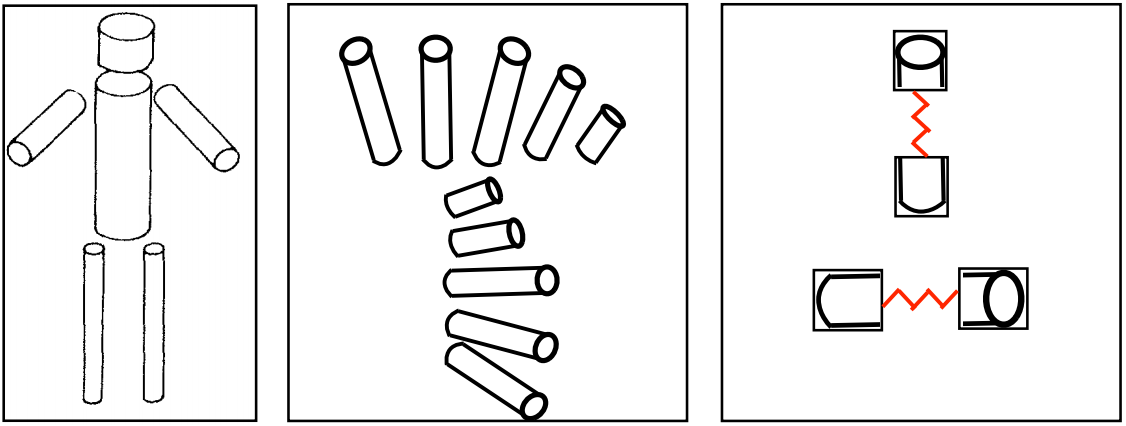
\includegraphics[width=8.3cm]{figure/pictorial.png}
  \caption{Illustration of the pictorial structure and mixture of local parts in Yang and Ramanan's paper \cite{Yang_PAMI2011}.}
\label{fig:pictorial}
\end{figure}

\begin{figure}[t]
  \begin{center}
      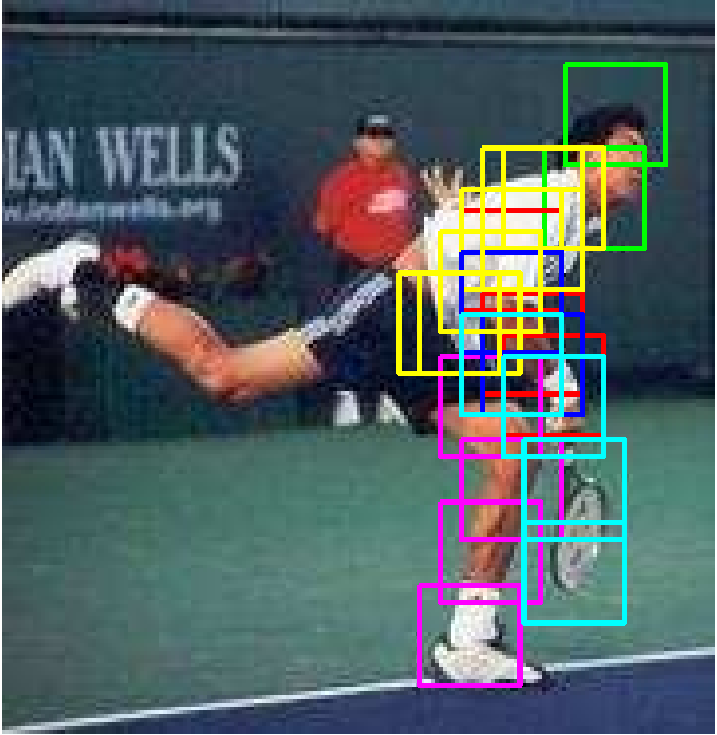
\includegraphics[height=0.22\linewidth]{figure/illustration/img0001_1.pdf}~~%&
      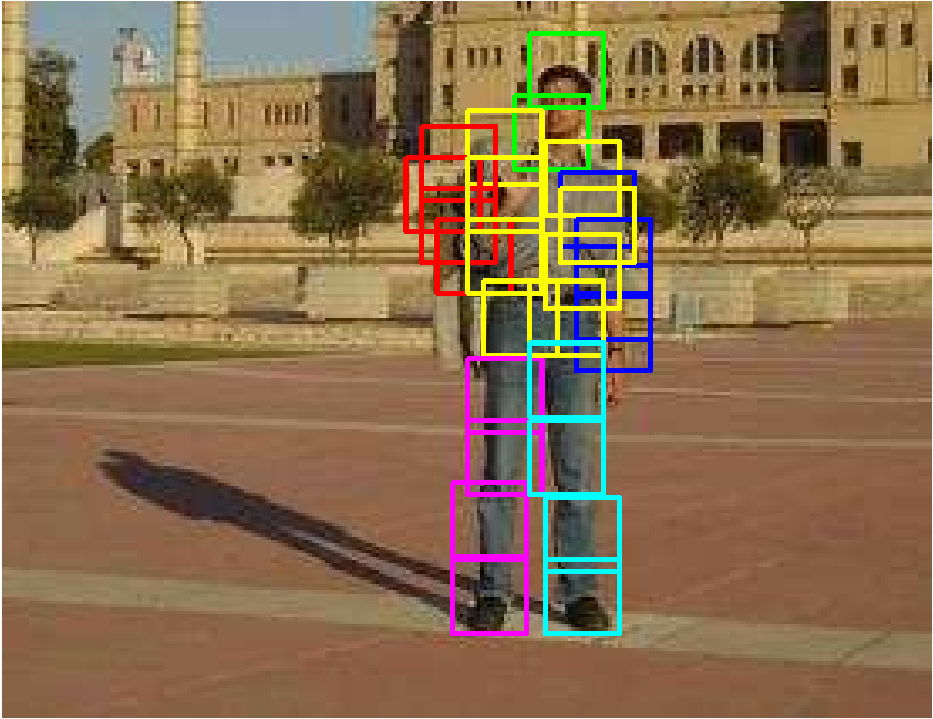
\includegraphics[height=0.22\linewidth]{figure/illustration/img0002_1.pdf}~~%&
      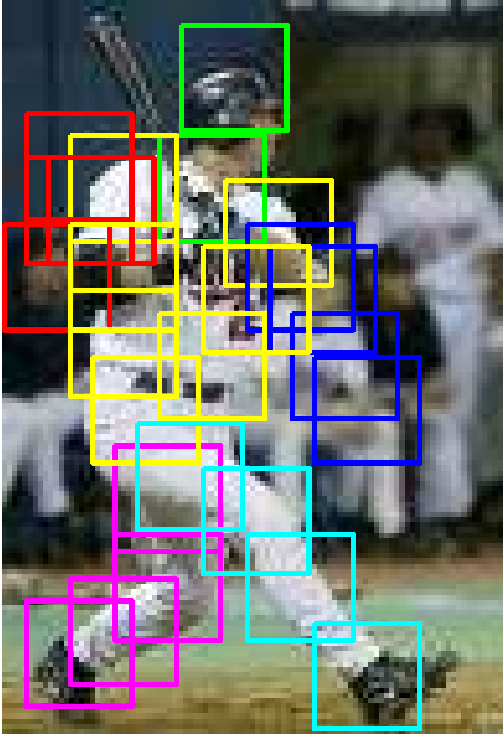
\includegraphics[height=0.22\linewidth]{figure/illustration/img0003_1.pdf}~~%&
      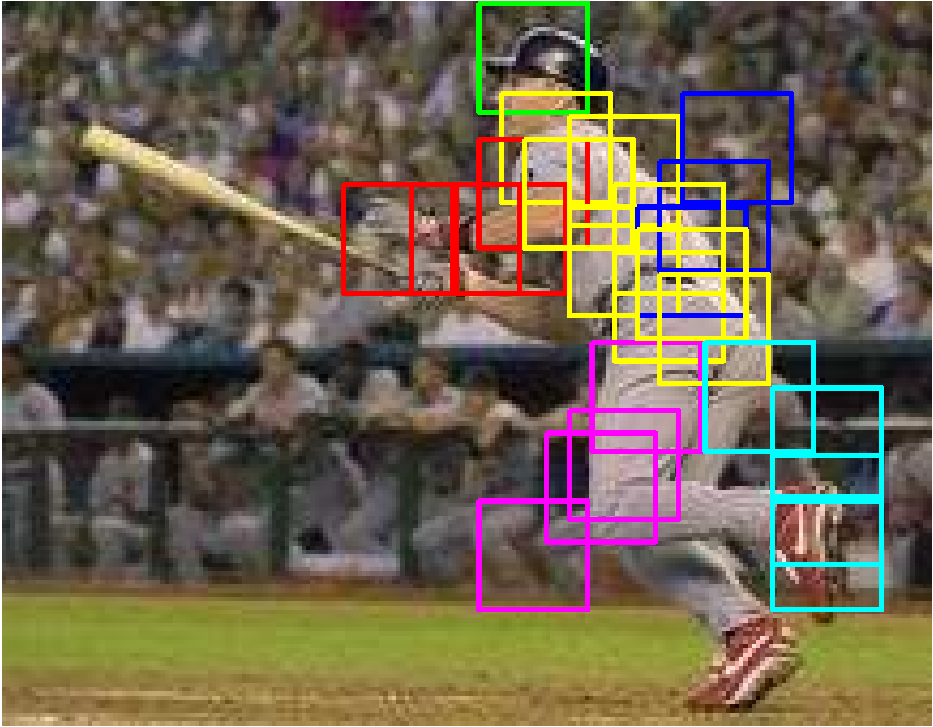
\includegraphics[height=0.22\linewidth]{figure/illustration/img0009_1.pdf}\\
      \vspace{0.2cm}
      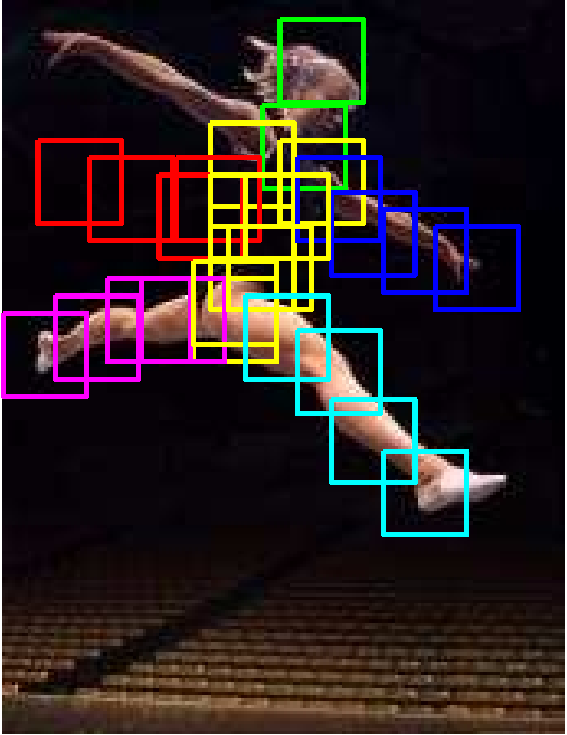
\includegraphics[height=0.24\linewidth]{figure/illustration/img0010_1.pdf}~~%&
      \includegraphics[height=0.24\linewidth]{figure/illustration/img0011_1.pdf}~~%&
      \includegraphics[height=0.24\linewidth]{figure/illustration/img0035_1.pdf}~~%&
      \includegraphics[height=0.24\linewidth]{figure/illustration/img0153_1.pdf}\\
      \vspace{0.2cm}
      \includegraphics[height=0.245\linewidth]{figure/illustration/img0097_1.pdf}~~%&
      \includegraphics[height=0.245\linewidth]{figure/illustration/img0105_1.pdf}~~%&
      \includegraphics[height=0.245\linewidth]{figure/illustration/img0112_1.pdf}~~%&
      \includegraphics[height=0.245\linewidth]{figure/illustration/img0046_1.pdf}\\
  \end{center}
  \caption{Illustration of Yang and Ramanan's work on human detection and pose estimation \cite{Yang_PAMI2011}. Different color of boxes identify different local parts of human body.}
\label{fig:intro}
\end{figure}

Our plan for this replication study can be divided into three main blocks. In short, we aim to first replicate the experimental results by following the techniques presented in the paper, and then study the proposed method further by experimenting with different settings, as well as understand how well it can be generalized to more realistic images.
\begin{itemize}
  \item Re-implement the inference algorithm, in paricular, the dymamic programming algorithm. This is a good starting point, since the authors have provided the code for learning and inference, and a fixed training and test split on the benchmark dataset. This will be helpful for us to verify the implementaion, since we can fix the trained model and focus only on the inference evaluation of the test set.
  \item Re-implement the learning algorithm, in particular, solving the structural SVM problem using the dual coordinate descent solver. The paper uses a fixed training set provided by the Image Parse dataset \cite{Ramanan_NIPS2006}. We plan to re-train the model by changing the size of the training set. The goal is to better understand how sensitive the trained model is to the size of the training set, and whether the current training set contains enough training samples. The training code is also provided by the author, so it can be used to verify our implementation.
  \item Build our own human dataset. We aim to build a small but more challenging dataset with more realistic images, and see how far can the target method go. This will also tell us 1) whether there is a bias in the dataset the paper evaluates on, and 2) how much gain could we get by adding new training image into the current training set.
\end{itemize}

We want to note that the authors have released their implementation for research purposes \footnote{http://www.ics.uci.edu/~yyang8/research/pose/}. This serves as a great resource for our replication study by the following reasons: 1) The information provided in the paper is insufficient from the full replcation aspect. For example, the paper describes their dual coordinate descent algorithm for learning only briefly and point to another reference. The reference does detail the algorithm better, but it could not provide some critical information in the context of the first paper such as initialization schemes, hyperparameters, and convergence criterions. Having the provided code will help us pick up the missing information. 2) The released code will provide a good amount of help (but not complete) to our debugging process. Instead of checking the whole framework due to incoherent outputs, we could compare the intermediate results to better understand what the mistakes are.

\begin{figure*}[t]
  \begin{center}
    %\begin{tabular}{cccccc}
      \includegraphics[height=0.133\linewidth]{figure/parse/00_img0036_1.pdf}~~%&
      \includegraphics[height=0.133\linewidth]{figure/parse/00_img0036_2.pdf}~~%&
      \includegraphics[height=0.133\linewidth]{figure/parse/00_img0017_1.pdf}~~%&
      \includegraphics[height=0.133\linewidth]{figure/parse/00_img0017_2.pdf}~~%&
      \includegraphics[height=0.133\linewidth]{figure/parse/00_img0086_1.pdf}~~%&
      \includegraphics[height=0.133\linewidth]{figure/parse/00_img0086_2.pdf}~~%&
      \includegraphics[height=0.133\linewidth]{figure/parse/00_img0029_1.pdf}~~%&
      \includegraphics[height=0.133\linewidth]{figure/parse/00_img0029_2.pdf}\\
%      \includegraphics[height=0.133\linewidth]{figure/parse/00_img0097_1.pdf}~~%&
%      \includegraphics[height=0.133\linewidth]{figure/parse/00_img0097_2.pdf}\\
      \vspace{0.2cm}
      \includegraphics[height=0.133\linewidth]{figure/parse/01_img0036_1.pdf}~~%&
      \includegraphics[height=0.133\linewidth]{figure/parse/01_img0036_2.pdf}~~%&
      \includegraphics[height=0.133\linewidth]{figure/parse/01_img0017_1.pdf}~~%&
      \includegraphics[height=0.133\linewidth]{figure/parse/01_img0017_2.pdf}~~%&
      \includegraphics[height=0.133\linewidth]{figure/parse/01_img0086_1.pdf}~~%&
      \includegraphics[height=0.133\linewidth]{figure/parse/01_img0086_2.pdf}~~%&
      \includegraphics[height=0.133\linewidth]{figure/parse/01_img0029_1.pdf}~~%&
      \includegraphics[height=0.133\linewidth]{figure/parse/01_img0029_2.pdf}\\
%      \includegraphics[height=0.133\linewidth]{figure/parse/01_img0097_1.pdf}~~%&
%      \includegraphics[height=0.133\linewidth]{figure/parse/01_img0097_2.pdf}\\
    %\end{tabular}
  \end{center}
  \caption{Qualitative samples of the inference replication on the Parse dataset. The pre-trained model is composed of 26 human parts. Each human detection is visualized by the detected bounding boxes of parts (left) and the skeletons (right). The top row show the result obtain from the author's implementation. The bottom row shows our implementation. Our implementation performs comparable to the authors' globally while there are local errors occasionally.}
  \label{fig:inference_exp}
\end{figure*}


\section{Inference}
We first briefly review the overall pictorial structure model for human detection proposed in \cite{Yang_PAMI2011} and the inference problem in Sec. \ref{sec:inference_ov}. Next we evaluate our implementation of the inference algorithm on the the Image Parse dataset \cite{Ramanan_NIPS2006} in Sec. \ref{sec:inference_eval}.

\subsection{Algorithm Overview}
\label{sec:inference_ov}
Yang and Ramanan proposed a pictorial structure representation to robustly model the human poses caused by articulated body configurations. They have a flexible design in the way that each local part is a mixture of different component (i.e. can be chosen from a template set). Let $I$ denote the image, $l_i = (x_i, y_i)$ be the location of part $i$, and $t_i$ be the mixture component of part $i$ (using the $t_i$th template for part $i$), where $i\in \{1,\dots,K\}$, $l_i\in\{1,\dots,L\}$, and $t_i\in\{1,\dots,T\}$. Assuming the human body is a tree structured graph $G=(V,E)$, the score function of a human is defined as following:
\begin{equation}
\label{eq:model}
  S(I,l,t) = \sum_{i\in V}\omega_i^{t_i}\cdot\phi(I,l_i) + \sum_{i,j\in E}\omega_{ij}^{t_i,t_j}\cdot\psi(l_i-l_j) + S(t).
\end{equation}
The three terms in eq. \ref{eq:model} correspond to the appearance model, deformation model, and the co-occurence model. Appreance model computes the local scores by placing a part template $w_i^{t_i}$ (of type $t_i$) at the location $i$. Deformation model controls the relative position of part $i$ and $j$. Note that $\psi(l_i-l_j)=[dx\text{~~}dx^{2}\text{~~}dy\text{~~}dy^{2}]^{\top}$. The co-occurrence model 
\begin{equation}
  S(t) = \sum_{i\in V}b_i^{t_i} + \sum_{i,j\in E}b_{ij}^{t_i,t_j}
\end{equation}
captures the occurrence likelihood of part $i$ with type $t_i$ and the co-occurrence likelihood of part $i$ with type $t_i$ and part $j$ with type $j$.

Given the model parameter, inference correspends to finding the maximum scoring locaions $(l,t)$ given the image $I$. Denote $z_i = (t_i,l_i)$, the eq \ref{eq:model} can be written as
\begin{equation}
  \begin{split}
    S(I,z) = & \sum_{i\in V}\phi_i(I,z_i) + \sum_{i,j\in E}\psi_{ij}(z_i,z_j), \\
    \text{where~~~~} & \phi_i(I,z_i) = \omega_i^{t_i}\cdot\phi(I,l_i)+b_i^{t_i} \\
                   & \psi_{ij}(z_i,z_j) = \omega_{ij}^{t_i,t_j}\cdot\psi(l_i-l_j)+b_{ij}^{t_i,t_j} \\
  \end{split}
  \label{eq:score}
\end{equation}
One nice consequence of the tree structure assumption on human body representation is enabling us to solve the optimization problem efficiently by dynamic programming. Our first focus of this replication study is on re-implementing this inference algorithm.

\subsection{Replication Result}
\label{sec:inference_eval}
We verify our implementation by first comparing the result on the same benchmark dataset, the Image Parse dataset \cite{Ramanan_NIPS2006}. The dataset consists of 100 training images and 205 test images. Since we only want to verify our inference implementation, we fix the trained model and use only the test images for evaluation. As \cite{Ramanan_NIPS2006} suggests, we evaluate the result based on the accuracy of body joint localization. We follow the paper and use two different metrics to measure such accuracy: 1) probability of a correct keypoint (PCK), and 2) average precision of keypoints (APK). Note that for PCK, the detector is ran within the annotated bounding box of the person. This metric highlights how well the body joints are localized given the ground-truth human bounding boxes. 

\begin{table}
  \begin{center}
    \begin{tabular}{|p{0.8cm}|p{0.5cm}|p{0.5cm}|p{0.5cm}|p{0.5cm}|p{0.5cm}|p{0.5cm}|p{0.5cm}||p{0.5cm}|}
      \hline
                              	 & Hea  & Sho  & Elb  & Wri  & Hip  & Kne  & Ank  & Avg  \\ \hline
      \hline
      \cite{Yang_PAMI2011} 	 & 88.3 & 81.7 & 62.2 & 42.0 & 71.0 & 68.5 & 61.2 & 67.8 \\ \hline
      Ours                    	 & 78.0 & 70.0 & 40.5 & 28.3 & 58.8 & 56.3 & 52.4 & 54.9 \\ \hline
    \end{tabular}
    \caption*{(a) Probability of correct keypoints (PCK)}
    \bigskip
    \begin{tabular}{|p{0.8cm}|p{0.5cm}|p{0.5cm}|p{0.5cm}|p{0.5cm}|p{0.5cm}|p{0.5cm}|p{0.5cm}||p{0.5cm}|}
      \hline
      	                      	 & Hea  & Sho  & Elb  & Wri  & Hip  & Kne  & Ank  & Avg \\ \hline
      \hline
      \cite{Yang_PAMI2011} 	 & 83.9 & 77.6 & 45.7 & 24.2 & 60.4 & 53.8 & 46.5 & 56.0 \\ \hline
      Ours                   	 & 69.3 & 60.7 & 24.5 & 10.4 & 42.3 & 36.6 & 33.6 & 39.6 \\ \hline
    \end{tabular}
    \caption*{(b) Average precision of keypoints (APK)}
  \end{center}
  \caption{We compare the inference result between the paper's implementation \cite{Yang_PAMI2011} and our implementation (Ours). The trained model is fixed to be the same. There is a accuracy drop in our implementation compared to the authors'.}
  \label{tab:parse_inf}
\end{table}

\begin{figure*}[t]
  \begin{center}
    %\begin{tabular}{cccccc}
      \includegraphics[height=0.123\linewidth]{figure/parse/00_img0011_1.pdf}~~%&
      \includegraphics[height=0.123\linewidth]{figure/parse/00_img0011_2.pdf}~~%&
      \includegraphics[height=0.123\linewidth]{figure/parse/00_img0098_1.pdf}~~%&
      \includegraphics[height=0.123\linewidth]{figure/parse/00_img0098_2.pdf}~~%&
      \includegraphics[height=0.123\linewidth]{figure/parse/00_img0156_1.pdf}~~%&
      \includegraphics[height=0.123\linewidth]{figure/parse/00_img0156_2.pdf}~~%&
      \includegraphics[height=0.123\linewidth]{figure/parse/00_img0163_1.pdf}~~%&
      \includegraphics[height=0.123\linewidth]{figure/parse/00_img0163_2.pdf}\\
      \vspace{0.2cm}
      \includegraphics[height=0.123\linewidth]{figure/parse/20_img0011_1.pdf}~~%&
      \includegraphics[height=0.123\linewidth]{figure/parse/20_img0011_2.pdf}~~%&
      \includegraphics[height=0.123\linewidth]{figure/parse/20_img0098_1.pdf}~~%&
      \includegraphics[height=0.123\linewidth]{figure/parse/20_img0098_2.pdf}~~%&
      \includegraphics[height=0.123\linewidth]{figure/parse/20_img0156_1.pdf}~~%&
      \includegraphics[height=0.123\linewidth]{figure/parse/20_img0156_2.pdf}~~%&
      \includegraphics[height=0.123\linewidth]{figure/parse/20_img0163_1.pdf}~~%&
      \includegraphics[height=0.123\linewidth]{figure/parse/20_img0163_2.pdf}\\
      \vspace{0.2cm}
      \includegraphics[height=0.123\linewidth]{figure/parse/21_img0011_1.pdf}~~%&
      \includegraphics[height=0.123\linewidth]{figure/parse/21_img0011_2.pdf}~~%&
      \includegraphics[height=0.123\linewidth]{figure/parse/21_img0098_1.pdf}~~%&
      \includegraphics[height=0.123\linewidth]{figure/parse/21_img0098_2.pdf}~~%&
      \includegraphics[height=0.123\linewidth]{figure/parse/21_img0156_1.pdf}~~%&
      \includegraphics[height=0.123\linewidth]{figure/parse/21_img0156_2.pdf}~~%&
      \includegraphics[height=0.123\linewidth]{figure/parse/21_img0163_1.pdf}~~%&
      \includegraphics[height=0.123\linewidth]{figure/parse/21_img0163_2.pdf}\\
    %\end{tabular}
  \end{center}
  \caption{Qualitative examples of the learning replication on the Parse dataset. The first row is using the authors' implementation for both learning and inference. The second row is using our implementation for learning and the authors' implementation for inference. The third row is using our implementation for both learning and inference. We obtain comparable results on learning when using the same inference implementation.}
  \label{fig:learning_exp}
\end{figure*}

We start by comparing our implementation and the implementation provided by the authors \footnote{Note that there is a slight difference between the result reported in the paper and the result we obtain from their code. We decide to use the output of the code for all the comparision in this study}. For the quantitative evaluation, we observe a significant drop (over $10\%$) in our implementation compared to the authors' implementation. We also show some qualitative examples in \ref{fig:inference_exp}, where the top rows are the results of the authors' implementation, while the bottom rows are ours. There are occationally errors in only a local part of the detection, for instance, the right arm on the leftmost image, and very few cases where there are global errors, for instance, the second left image. Since in general our implementation works in a reasonable level from a qualitative perspect, it suggests that the cause of the gap between our result and the original paper is less likely to be on the algorithmic side. Unfortunately, the question remains at the due of this report. We suggest a few possible explains on the result difference: 1) There could be a bug caused by a typo in our implementation, and it has a local affect which does not reflect significantly in the global detection result. 2) There could possibly be a numerical issue on the computation, which suggests that the implementation is not numerically stable. From the debugging experience, we learned that the debugging can still be difficult and time-consuming even the original code is available.

%\begin{table}[t]
%  \begin{center}
%    \begin{tabular}{|p{0.8cm}|p{0.5cm}|p{0.5cm}|p{0.5cm}|p{0.5cm}|p{0.5cm}|p{0.5cm}|p{0.5cm}||p{0.5cm}|}
%      \hline
%      Parse                & Hea  & Sho  & Elb  & Wri  & Hip  & Kne  & Ank  & Avg  \\ \hline
%      \hline
%      \cite{Yang_PAMI2011} & 88.3 & 82.7 & 61.2 & 44.1 & 68.8 & 66.8 & 61.0 & 67.6 \\ \hline
%      Mine                 & 77.3 & 71.2 & 47.3 & 31.7 & 58.8 & 56.8 & 49.3 & 56.1 \\ \hline
%    \end{tabular}
%  \end{center}
%  \caption{Probability of correct keypoints (PCK) on the Image Parse Dataset.}
%  \label{tab:pck_parse}
%\end{table}

%\begin{table}
%  \begin{center}
%    \begin{tabular}{|p{0.8cm}|p{0.5cm}|p{0.5cm}|p{0.5cm}|p{0.5cm}|p{0.5cm}|p{0.5cm}|p{0.5cm}||p{0.5cm}|}
%      \hline
%      Parse                & Hea  & Sho  & Elb  & Wri  & Hip  & Kne  & Ank  & Avg \\ \hline
%      \hline
%      \cite{Yang_PAMI2011} & 83.9 & 77.0 & 49.6 & 26.8 & 56.1 & 52.3 & 43.7 & 55.6 \\ \hline
%      Mine                 & 71.2 & 62.8 & 32.4 & 15.8 & 42.9 & 38.8 & 33.1 & 42.4 \\ \hline
%    \end{tabular}
%  \end{center}
%  \caption{Average precision of keypoints (APK) on the Image Parse Dataset.}
%  \label{tab:apk_parse}
%\end{table}

%\section{Target Questions}
%{\color{blue}
%\begin{enumerate}
%  \item Why is your target paper important enough for the effort of replication?
%  \item How will your replication benefit the state of the art?  Will this increase (or decrease) our confidence in a method that can advance the state of the art?  Did their paper and their other resources provide the information you needed to do a replication.
%  \item What did you actually have to do, to get the replication working?  Did you replicate the entire work? Did you extend their work?
%  \item How did you evaluate what you did?  How do you know how well your replication worked?
%  \item What is the significance of your results, in terms of the confidence we can have in the results of the target article and in its authors?  Does your replication help advance the state of the art?  Are there new insights into the original article's problem or its solution, that you got from your replication effort and that would be valuable to the reader?
%\end{enumerate}
%}


\section{Learning}
The goal is to learn the model parameters in \ref{eq:score} that maximizes the discrimination power. The paper formulates a structural SVM learning problem and solves it using an efficient algorithm based on dual coordinate descent (DCD). The primary focus of our replication study is to re-implement the dual coordinate descent solver. We first review the learning problem and the DCD solver in Sec \ref{sec:learning_ov}. The replication result is presented in Sec \ref{sec:learning_rep}. 

\subsection{Algorithm Overview}
\label{sec:learning_ov}
The paper adopts a supervised learning paradign. Given labeled positive examples $\{I_n,l_n,t_n\}$ (images with labeled human body parts) and negative examples $\{I_n\}$, the goal is to learn a discriminative model that will score high on test regions when a person is presented and score low otherwise. Since the score function \ref{eq:score} is linear in model parameters $\beta=(\omega,b)$, we can write $S(I,z)=\beta\cdot\Phi(I,z)$. The model parameters is then learnt by solving the following optimization problem:
\begin{equation}
  \begin{split}
    \arg\min_{\beta,\xi_n\geq0}                      ~~~& \frac{1}{2}||\beta||^2+C\sum_n{\xi_n} \\
    \text{s.t.}~~ \forall n\in \text{pos}            ~~~& \beta^{T}\Phi(I_n,z_n) \geq 1-\xi_n \\
                  \forall n\in \text{neg}, \forall z ~~~& \beta^{T}\Phi(I_n,z) \leq -1+\xi_n,
  \end{split}
\label{eq:ssvm}
\end{equation}
where $C$ is the hyperparameter and $\xi_n$ is the slack variable corresponded to sample $n$.

The form of the learning problem above is known as a structural SVM (SSVM), an extension of the binary SVM to handle the prediction of structured outputs. There has been many powerful techniques proposed to solve the SSVM problem, for instance, the cutting plane algorithm and the stochastic gradient descent (SGD). This paper uses a {\it dual coordinate descent } solver, which is detailed in \cite{Ramanan_TR2012} by one of the co-authors. As \cite{Ramanan_TR2012} mentioned, in large scale learning problems, batch algorithms are often impractical due to the difficulty of fitting the entire dataset into the memory, while the online algorithms alleviate such problem but often converge slowly. The proposed dual coordinate descent solver serves as an intermediate solution: it keeps a relatively small set of active constraints (support vectors) in the memory, which leads to a better performance on the convergence, while keeping it as stable as the batch algorithms.

The proposed dual coordinate descent solver has many practical advantages in large scale learning problems, and it could potentially be benefitial to our later research studies. Thus we decide to focus primarily on implementing the proposed DCD algorithm for the training part of this replication study. 

\begin{table}
  \begin{adjustwidth}{-0.3cm}{}
  \begin{center}
    \begin{tabular}{|p{1.1cm}|p{0.5cm}|p{0.5cm}|p{0.5cm}|p{0.5cm}|p{0.5cm}|p{0.5cm}|p{0.5cm}||p{0.5cm}|}
      \hline
      	                	                         & Hea  & Sho  & Elb  & Wri  & Hip  & Kne  & Ank  & Avg  \\ \hline
      \hline
      \cite{Yang_PAMI2011} / \cite{Yang_PAMI2011} 	 & 88.3 & 81.7 & 62.2 & 42.0 & 71.0 & 68.5 & 61.2 & 67.8 \\ \hline
      O / \cite{Yang_PAMI2011}			  	 & 87.3 & 79.8 & 58.8 & 43.7 & 70.0 & 63.9 & 58.3 & 66.0 \\ \hline
      O / O			 		 	 & 79.0 & 71.7 & 40.7 & 30.0 & 57.8 & 58.3 & 54.1 & 56.0 \\ \hline
    \end{tabular}
    \caption*{Probability of correct keypoints (PCK).}
    \bigskip
    \begin{tabular}{|p{1.1cm}|p{0.5cm}|p{0.5cm}|p{0.5cm}|p{0.5cm}|p{0.5cm}|p{0.5cm}|p{0.5cm}||p{0.5cm}|}
      \hline
                                                    	 & Hea  & Sho  & Elb  & Wri  & Hip  & Kne  & Ank  & Avg \\ \hline
      \hline
      \cite{Yang_PAMI2011} / \cite{Yang_PAMI2011} 	 & 83.9 & 77.6 & 45.7 & 24.2 & 60.4 & 53.8 & 46.5 & 56.0 \\ \hline
      O / \cite{Yang_PAMI2011}			 	 & 83.2 & 75.7 & 44.9 & 26.5 & 57.0 & 49.2 & 41.9 & 54.1 \\ \hline
      O / O			 			 & 72.5 & 63.6 & 25.1 & 13.8 & 42.7 & 43.0 & 37.1 & 42.5 \\ \hline
    \end{tabular}
    \caption*{Average precision of keypoints (APK).}
  \end{center}
  \end{adjustwidth}
  \caption{We compare the result of learning between the paper's implementation and our implementation. A / B represents using A for learning and B for inference (\cite{Yang_PAMI2011} for the paper and O for Ours). We achive comparable results on learning when using the same inference implementation. Our inference implementation causes a performance drop as in Tab. \ref{tab:parse_inf}.}
  \label{tab:parse_learn}
\end{table}

Now we highlight the idea of the proposed DCD solver (refer to \cite{Ramanan_TR2012} for the complete details). The optimization problem \ref{eq:ssvm} is a quadratic programming (QP), and we can derive the associated Lagrangian:
\begin{equation}
  \begin{split}
  L(\beta,\xi,\alpha,\mu) = & \frac{1}{2}||\beta||^2+C\sum_i\xi_i-\sum_{ij}\alpha_{ij}(\beta^{T}\Phi-1+\xi_i) \\
                            & -\sum_{i}\mu_i\xi_i,
  \end{split}
\end{equation}
where $\alpha$ and $\mu$ are the Lagrange multipliers. We can take the derivatives of the Lagragian with respect to the primal variables, and get the dual of the QP in \ref{eq:ssvm}:
\begin{equation}
  \begin{split}
  \max_{\alpha\geq0,\mu\geq0} ~~~F(\alpha) = - & \frac{1}{2}\sum_{ij,kl}\alpha_{ij}x^{T}_{ij}x_{kl}\alpha_{kl}+\sum_{ij}\alpha_{ij} \\
  \text{s.t.}~~ \forall i, ~~~& \sum_{j}\alpha_{ij}\leq 1 \\
  %\forall i,j,             ~~~&\alpha_{ij}\geq 0.
  \end{split}
\label{eq:dual}
\end{equation}
By strong dualality, the solution of problem \ref{eq:ssvm} (primal) and problem \ref{eq:dual} (dual) are equivalent. One important property about \ref{eq:dual} is that when we minimize the objective with respect to a single $\alpha_{ij}$ while keeping other fixed, the objective function is quadratic over $\alpha_i$, and there exists an analytical solution. The efficiency of the proposed DCD algorithm is thus based on this fact. We randomly pick a single $\alpha_{ij}$ and optimize \ref{eq:dual}, and this will garuantee to increase the object function. It is also shown in \cite{Ramanan_TR2012} that the lower-bound and an approximated upper-bound can be tracked efficiently during the run of the optimization. We can determine the convergence of the learning when the gap between the upper-bound and the lower-bound is below a fixed threshold.

\begin{figure}[t]
  \center
  \includegraphics[width=0.90\linewidth]{figure/train_num.pdf}
  \caption{Evaluation on Parse test set using different number of training images.}
  \label{fig:train_num}
\end{figure}

\subsection{Replication Result}
\label{sec:learning_rep}

We use the standard training and test split for the Image Parse dataset. We compare the result obtained by 1) using the authors' implementation for both learning and inference, 2) using our implementation for learning and the authors' implementation for inference, and 3) use our implementation for both learning and training. We report the body joint localization accuracies and qualitative examples in Tab. \ref{tab:parse_inf} and Fig. \ref{fig:inference_exp}, respectively. As shown in Tab. \ref{tab:parse_inf}, we obtain comparable result with the authors' implementation when the inference choice is fixed. This indicates a success in the replication on the learning side, since our implementation performs comparable to the authors' implementation. However, we still see an accuracy drop when applying our inference implementation. This is expected from the result in Sec \ref{sec:inference_eval}. We note that the success of the replication is contributed significantly from the availability of the paper's code. The code provides large amount of additional information to the paper, especially on the learning side, such as the initialization scheme, loading control of data sequence, and hyperparameters.

We also investigate the affect of the size of the training set on the Parse dataet. We change the number of number of training images by randomly picking a subset of the original training set, and run the test experiment on the test set. The results on PCK and APK are shown in Fig. \ref{fig:train_num}. We observe that the accuracy converges around using 80 training images. The reason could be that the Parse dataset is relatively small and the statistics of the training and test set are similar. Therefore, using a small amount of training images can reach the upper bound of the test accuracy. As we will shown in Sec \ref{sec:newdata}, the statistics of the Parse dataset is very different from the general images we take everyday. To increase the generalization power of the trained model, we need to add the training images from different sources to balance the statistics of the dataset, in order to increase the generalization power.

\begin{figure}[t]
  \center
  \includegraphics[width=0.9\linewidth]{figure/newdata.jpg}
  \caption{Our proposed new dataset. It contains 70 images taken from our daily life.}
  \label{fig:newdata}
\end{figure}

\section{New Dataset}
\label{sec:newdata}

To better understand the result on the parse dataset, as well as to gain more insights on the generalization of the trained model, we propose a new dataset for further evaluations. As shown in Fig. \ref{fig:newdata}, this dataset contains 70 images which mostly came from the photos we took in our past daily life. Compared to the images in the Parse dataset, which are carefully selected for evaluation purposes, our new dataset are more common and realistic. We annotate the human body joints for the new dataset in the same way as the parse dataset. 

\begin{table}[t]
  \begin{center}
    \begin{tabular}{|p{1.1cm}|p{0.5cm}|p{0.5cm}|p{0.5cm}|p{0.5cm}|p{0.5cm}|p{0.5cm}|p{0.5cm}||p{0.5cm}|}
      \hline
      		            	                         & Hea  & Sho  & Elb  & Wri  & Hip  & Kne  & Ank  & Avg  \\ \hline
      \hline
      \cite{Yang_PAMI2011} / \cite{Yang_PAMI2011} 	 & 67.9 & 47.9 & 29.3 & 20.7 & 33.6 & 31.4 & 30.0 & 37.2 \\ \hline
      \cite{Yang_PAMI2011} / O                   	 & 60.0 & 39.3 & 17.9 & 19.3 & 25.0 & 25.7 & 30.7 & 31.1 \\ \hline
      O / \cite{Yang_PAMI2011}			 	 & 67.9 & 51.4 & 22.9 & 18.6 & 34.3 & 30.7 & 31.4 & 36.7 \\ \hline
      O / O			 		 	 & 57.9 & 38.6 & 20.7 & 15.0 & 24.3 & 27.1 & 32.1 & 30.8 \\ \hline
    \end{tabular}
    \caption*{Probability of correct keypoints (PCK).}
    \bigskip
    \begin{tabular}{|p{1.1cm}|p{0.5cm}|p{0.5cm}|p{0.5cm}|p{0.5cm}|p{0.5cm}|p{0.5cm}|p{0.5cm}||p{0.5cm}|}
      \hline
      		                                         & Hea  & Sho  & Elb  & Wri  & Hip  & Kne  & Ank  & Avg \\ \hline
      \hline
      \cite{Yang_PAMI2011} / \cite{Yang_PAMI2011}	 & 54.8 & 35.0 & 19.4 & 10.5 & 22.0 & 15.7 & 19.1 & 25.2 \\ \hline
      \cite{Yang_PAMI2011} / O                   	 & 46.2 & 29.0 &  9.6 &  6.5 & 19.8 & 15.0 & 17.3 & 20.5 \\ \hline
      O / \cite{Yang_PAMI2011}			 	 & 49.6 & 34.5 & 15.7 &  7.6 & 22.8 & 13.9 & 18.0 & 23.2 \\ \hline
      O / O			 			 & 47.9 & 32.3 &  8.0 &  4.5 & 15.1 & 14.6 & 19.6 & 20.3 \\ \hline
    \end{tabular}
    \caption*{Average precision of keypoints (APK).}
  \end{center}
  \caption{The inference result on the new dataset using the model trainined on the Parse dataset. The result of different implemention choices are reported. A / B represents using A for learning and B for inference (\cite{Yang_PAMI2011} for the paper and O for Ours). The performance drops significantly compared to the Parse test set.}
  \label{tab:newdata_acc}
\end{table} 

\begin{figure*}[t]
  \begin{center}
    %\begin{tabular}{cccccc}
      \includegraphics[height=0.117\linewidth]{figure/new_dataset/img0017_1.pdf}~~%&
      \includegraphics[height=0.117\linewidth]{figure/new_dataset/img0017_2.pdf}~~%&
      \includegraphics[height=0.117\linewidth]{figure/new_dataset/img0023_1.pdf}~~%&
      \includegraphics[height=0.117\linewidth]{figure/new_dataset/img0023_2.pdf}~~%&
      \includegraphics[height=0.117\linewidth]{figure/new_dataset/img0063_1.pdf}~~%&
      \includegraphics[height=0.117\linewidth]{figure/new_dataset/img0063_2.pdf}~~%&
      \includegraphics[height=0.117\linewidth]{figure/new_dataset/img0058_1.pdf}~~%&
      \includegraphics[height=0.117\linewidth]{figure/new_dataset/img0058_2.pdf}\\
      \vspace{0.2cm}
      \includegraphics[height=0.111\linewidth]{figure/new_dataset/img0018_1.pdf}~~%&
      \includegraphics[height=0.111\linewidth]{figure/new_dataset/img0018_2.pdf}~~%&
      \includegraphics[height=0.111\linewidth]{figure/new_dataset/img0010_1.pdf}~~%&
      \includegraphics[height=0.111\linewidth]{figure/new_dataset/img0010_2.pdf}~~%&
      \includegraphics[height=0.111\linewidth]{figure/new_dataset/img0035_1.pdf}~~%&
      \includegraphics[height=0.111\linewidth]{figure/new_dataset/img0035_2.pdf}~~%&
      \includegraphics[height=0.111\linewidth]{figure/new_dataset/img0014_1.pdf}~~%&
      \includegraphics[height=0.111\linewidth]{figure/new_dataset/img0014_2.pdf}\\
    %\end{tabular}
  \end{center}
  \caption{Qualitative examples on the new dataset using the model trainined on the Parse dataset.}
  \label{fig:newdata_exp}
\end{figure*}

To see how well the model trained on the Parse dataset generalizes to images from a different source, we take our trained model from Sec \ref{sec:learning_rep} and run inference on the new dataset. The accuracies of body part localization (PCK and APK) are shown in Table \ref{tab:newdata_acc}. In addition to the same drop of performance for our inference implementation, the overall accuracies drops significantly compare to the evaluation on the Parse dataset (Table \ref{tab:parse_inf} and \ref{tab:parse_learn}). This indicates there is a bias between the Parse dataset and our new dataset. We point out four major issues that explains the accuracy drop on the new dataset as follows. 1) {\bf Poses:} Most images in the Parse dataset are people playing sports, e.g. basketball, baseball, tennis, etc. This causes a bias in the pose distribution. For example, the model learnt from the Parse dataset can not identify the squating pose shown in the lower left image in Fig \ref{fig:newdata_exp} because of lacking similar training examples. 2) {\bf Focus of Image:} People are often the dominant objects of the images in the Parse dataset. This is not necessarily true for general images, as seen in Fig \ref{fig:newdata_exp}. The problem becomes significant when the scale of the person is too small such that the extracted feature can not discriminate difference poses. 3) {\bf Occlusion:} Images in Parse have been selected to limit the amount of occlusions and self-occlusions. The limbs can be observed most of the time possibly due to the performed activity (sports). However, in a more realisitic scenario, human in an image suffers more from occlusions and self-occlusions. In many cases, half of the body may not be visible at all. Unfortunately the proposed method are not capable of handling these cases yet. 4) {\bf Noisy Background:} The background of the human can be very cluttered in realistic images. The problem is even significant when the people are less dominant in the image. As shown in the lower right image of Fig \ref{fig:newdata_exp}, noisy background can cause false positives due to the noisy image features. From the analysis above, we conclude that there is still a gap between the Parse dataset and realistic images, and the later is still very challenging for several reasons that may cause the proposed method to fail.

\section{Conclusion}
In this replication study, we have re-implemented the inference algorithm and the learning algorithm. The replication of learning is successful, while the replication of inference still requires verfication. We show some analysis on how training on the Parse dataset is affected by the size of the training set. We also perform extensive studies on the generalizaion of the trained model by testing it on a new proposed dataset. We conclude that due to the large variability of human body poses, as well as different sources of noises in the real-world images, a large amount of training images is required to successfully increase the generalization power of the proposed method.

\begin{figure}[t]
  \begin{center}
    %\begin{tabular}{cccccc}
      \includegraphics[height=0.43\linewidth]{figure/anecdotal/img0002_2.pdf}~~%&
      \includegraphics[height=0.43\linewidth]{figure/anecdotal/img0003_2.pdf}~~%&
      \includegraphics[height=0.43\linewidth]{figure/anecdotal/img0005_2.pdf}\\
      \vspace{0.2cm}
      \includegraphics[height=0.32\linewidth]{figure/anecdotal/img0006_2.pdf}~~%&
      \includegraphics[height=0.32\linewidth]{figure/anecdotal/img0007_2.pdf}\\
    %\end{tabular}
  \end{center}
  \caption{Anecdotal examples on non-human (or fake human) images.}
  \label{fig:newdata_anec}
\end{figure}

%\section{Milestone}
%\label{}

%\begin{figure*}[t]
%  \centering
%  \includegraphics[width=17.3cm]{figure/templates.png}
%  \caption{Visualization of the learned model.}
%\label{}
%\end{figure*}

%The milestones are shown in Table \ref{tab:6}
%\begin{table}[t]
%  \centering
%  \begin{tabular}{|l|p{5.5 cm}|}
%    \hline
%    Date          & Plan \\
%    \hline
%    02.05 - 02.11 & re-implement the inference algorithm \\
%    02.12 - 02.18 & re-implement the inference algorithm \\
%    02.19 - 02.25 & re-implement the inference algorithm \\
%                  & compare the result with the paper \\
%                  & analyze the result \\
%    02.25 - 03.04 & re-do training \\
%    03.05 - 03.11 & re-do training \\
%    03.12 - 03.18 & collect new dataset \\
%    03.19 - 03.25 & collect new dataset \\
%    03.26 - 04.01 & run experiment on new dataset \\
%    04.02 - 04.08 & run experiment on new dataset \\
%    04.09 - 04.15 & Buffer time \\
%    04.16 - 04.21 & Prepare for presentation \\
%    \hline
%  \end{tabular}
%  \caption{Project milestones}
%  \label{tab:6}
%\end{table}

%%%%%%%%% ABSTRACT
%\begin{abstract}
%   The ABSTRACT is to be in fully-justified italicized text, at the top
%   of the left-hand column, below the author and affiliation
%   information. Use the word ``Abstract'' as the title, in 12-point
%   Times, boldface type, centered relative to the column, initially
%   capitalized. The abstract is to be in 10-point, single-spaced type.
%   Leave two blank lines after the Abstract, then begin the main text.
%   Look at previous CVPR abstracts to get a feel for style and length.
%\end{abstract}

%%%%%%%%% BODY TEXT
%\section{Introduction}
%
%Please follow the steps outlined below when submitting your manuscript to
%the IEEE Computer Society Press.  This style guide now has several
%important modifications (for example, you are no longer warned against the
%use of sticky tape to attach your artwork to the paper), so all authors
%should read this new version.
%
%%-------------------------------------------------------------------------
%\subsection{Language}
%
%All manuscripts must be in English.
%
%\subsection{Dual submission}
%
%By submitting a manuscript to CVPR, the authors guarantee that it has
%not been previously published or accepted for publication in substantially
%similar form in an archival peer-reviewed forum. Furthermore, no paper which
%contains significant overlap with the contributions of this paper is neither
%under review at the moment of submission nor will be submitted during the
%CVPR 2013 review period to {\bf any of the following}: another conference,
%a workshop, or a journal. The authors also attest that they did not submit
%substantially similar submissions to CVPR 2013. {\bf Violation of any of
%these conditions will lead to rejection.} If you are not sure about the
%extent of overlap, you may upload a copy of the paper in question as
%supplementary material. Note that a Technical Report (departmental,
%arXiv.org, etc.) that is put up without any form of direct peer-review is
%{\bf NOT} considered a publication. Likewise, mention of the work under
%review in a presentation is {\bf NOT} considered a violation.
%
%If there are papers that may appear to the reviewers
%to violate this condition, then it is your responsibility to: (1)~cite
%these papers (preserving anonymity as described in Section 1.6 below),
%(2)~argue in the body of your paper why your CVPR paper is non-trivially
%different from these concurrent submissions, and (3)~include anonymized
%versions of those papers in the supplemental material.
%
%\subsection{Paper length}
%CVPR papers may be between 6 pages and 8 pages, with a \$100 per page added
%fee.  Overlength papers will simply not be reviewed.  This includes papers
%where the margins and formatting are deemed to have been significantly
%altered from those laid down by this style guide.  Note that this
%\LaTeX\ guide already sets figure captions and references in a smaller font.
%The reason such papers will not be reviewed is that there is no provision for
%supervised revisions of manuscripts.  The reviewing process cannot determine
%the suitability of the paper for presentation in eight pages if it is
%reviewed in eleven.  If you submit 8 for review expect to pay the added page
%charges for them.
%
%%-------------------------------------------------------------------------
%\subsection{The ruler}
%The \LaTeX\ style defines a printed ruler which should be present in the
%version submitted for review.  The ruler is provided in order that
%reviewers may comment on particular lines in the paper without
%circumlocution.  If you are preparing a document using a non-\LaTeX\
%document preparation system, please arrange for an equivalent ruler to
%appear on the final output pages.  The presence or absence of the ruler
%should not change the appearance of any other content on the page.  The
%camera ready copy should not contain a ruler. (\LaTeX\ users may uncomment
%the \verb'\cvprfinalcopy' command in the document preamble.)  Reviewers:
%note that the ruler measurements do not align well with lines in the paper
%--- this turns out to be very difficult to do well when the paper contains
%many figures and equations, and, when done, looks ugly.  Just use fractional
%references (e.g.\ this line is $095.5$), although in most cases one would
%expect that the approximate location will be adequate.
%
%\subsection{Mathematics}
%
%Please number all of your sections and displayed equations.  It is
%important for readers to be able to refer to any particular equation.  Just
%because you didn't refer to it in the text doesn't mean some future reader
%might not need to refer to it.  It is cumbersome to have to use
%circumlocutions like ``the equation second from the top of page 3 column
%1''.  (Note that the ruler will not be present in the final copy, so is not
%an alternative to equation numbers).  All authors will benefit from reading
%Mermin's description of how to write mathematics:
%\url{http://www.pamitc.org/documents/mermin.pdf}.
%
%
%\subsection{Blind review}
%
%Many authors misunderstand the concept of anonymizing for blind
%review.  Blind review does not mean that one must remove
%citations to one's own work---in fact it is often impossible to
%review a paper unless the previous citations are known and
%available.
%
%Blind review means that you do not use the words ``my'' or ``our''
%when citing previous work.  That is all.  (But see below for
%techreports)
%
%Saying ``this builds on the work of Lucy Smith [1]'' does not say
%that you are Lucy Smith, it says that you are building on her
%work.  If you are Smith and Jones, do not say ``as we show in
%[7]'', say ``as Smith and Jones show in [7]'' and at the end of the
%paper, include reference 7 as you would any other cited work.
%
%An example of a bad paper just asking to be rejected:
%\begin{quote}
%\begin{center}
%    An analysis of the frobnicatable foo filter.
%\end{center}
%
%   In this paper we present a performance analysis of our
%   previous paper [1], and show it to be inferior to all
%   previously known methods.  Why the previous paper was
%   accepted without this analysis is beyond me.
%
%   [1] Removed for blind review
%\end{quote}
%
%
%An example of an acceptable paper:
%
%\begin{quote}
%\begin{center}
%     An analysis of the frobnicatable foo filter.
%\end{center}
%
%   In this paper we present a performance analysis of the
%   paper of Smith \etal [1], and show it to be inferior to
%   all previously known methods.  Why the previous paper
%   was accepted without this analysis is beyond me.
%
%   [1] Smith, L and Jones, C. ``The frobnicatable foo
%   filter, a fundamental contribution to human knowledge''.
%   Nature 381(12), 1-213.
%\end{quote}
%
%If you are making a submission to another conference at the same time,
%which covers similar or overlapping material, you may need to refer to that
%submission in order to explain the differences, just as you would if you
%had previously published related work.  In such cases, include the
%anonymized parallel submission~\cite{Authors13} as additional material and
%cite it as
%\begin{quote}
%[1] Authors. ``The frobnicatable foo filter'', F\&G 2013 Submission ID 324,
%Supplied as additional material {\tt fg324.pdf}.
%\end{quote}
%
%Finally, you may feel you need to tell the reader that more details can be
%found elsewhere, and refer them to a technical report.  For conference
%submissions, the paper must stand on its own, and not {\em require} the
%reviewer to go to a techreport for further details.  Thus, you may say in
%the body of the paper ``further details may be found
%in~\cite{Authors13b}''.  Then submit the techreport as additional material.
%Again, you may not assume the reviewers will read this material.
%
%Sometimes your paper is about a problem which you tested using a tool which
%is widely known to be restricted to a single institution.  For example,
%let's say it's 1969, you have solved a key problem on the Apollo lander,
%and you believe that the CVPR70 audience would like to hear about your
%solution.  The work is a development of your celebrated 1968 paper entitled
%``Zero-g frobnication: How being the only people in the world with access to
%the Apollo lander source code makes us a wow at parties'', by Zeus \etal.
%
%You can handle this paper like any other.  Don't write ``We show how to
%improve our previous work [Anonymous, 1968].  This time we tested the
%algorithm on a lunar lander [name of lander removed for blind review]''.
%That would be silly, and would immediately identify the authors. Instead
%write the following:
%\begin{quotation}
%\noindent
%   We describe a system for zero-g frobnication.  This
%   system is new because it handles the following cases:
%   A, B.  Previous systems [Zeus et al. 1968] didn't
%   handle case B properly.  Ours handles it by including
%   a foo term in the bar integral.
%
%   ...
%
%   The proposed system was integrated with the Apollo
%   lunar lander, and went all the way to the moon, don't
%   you know.  It displayed the following behaviours
%   which show how well we solved cases A and B: ...
%\end{quotation}
%As you can see, the above text follows standard scientific convention,
%reads better than the first version, and does not explicitly name you as
%the authors.  A reviewer might think it likely that the new paper was
%written by Zeus \etal, but cannot make any decision based on that guess.
%He or she would have to be sure that no other authors could have been
%contracted to solve problem B.
%
%FAQ: Are acknowledgements OK?  No.  Leave them for the final copy.
%
%
%\begin{figure}[t]
%\begin{center}
%\fbox{\rule{0pt}{2in} \rule{0.9\linewidth}{0pt}}
%   %\includegraphics[width=0.8\linewidth]{egfigure.eps}
%\end{center}
%   \caption{Example of caption.  It is set in Roman so that mathematics
%   (always set in Roman: $B \sin A = A \sin B$) may be included without an
%   ugly clash.}
%\label{fig:long}
%\label{fig:onecol}
%\end{figure}
%
%\subsection{Miscellaneous}
%
%\noindent
%Compare the following:\\
%\begin{tabular}{ll}
% \verb'$conf_a$' &  $conf_a$ \\
% \verb'$\mathit{conf}_a$' & $\mathit{conf}_a$
%\end{tabular}\\
%See The \TeX book, p165.
%
%The space after \eg, meaning ``for example'', should not be a
%sentence-ending space. So \eg is correct, {\em e.g.} is not.  The provided
%\verb'\eg' macro takes care of this.
%
%When citing a multi-author paper, you may save space by using ``et alia'',
%shortened to ``\etal'' (not ``{\em et.\ al.}'' as ``{\em et}'' is a complete word.)
%However, use it only when there are three or more authors.  Thus, the
%following is correct: ``
%   Frobnication has been trendy lately.
%   It was introduced by Alpher~\cite{Alpher02}, and subsequently developed by
%   Alpher and Fotheringham-Smythe~\cite{Alpher03}, and Alpher \etal~\cite{Alpher04}.''
%
%This is incorrect: ``... subsequently developed by Alpher \etal~\cite{Alpher03} ...''
%because reference~\cite{Alpher03} has just two authors.  If you use the
%\verb'\etal' macro provided, then you need not worry about double periods
%when used at the end of a sentence as in Alpher \etal.
%
%For this citation style, keep multiple citations in numerical (not
%chronological) order, so prefer \cite{Alpher03,Alpher02,Authors13} to
%\cite{Alpher02,Alpher03,Authors13}.
%
%
%\begin{figure*}
%\begin{center}
%\fbox{\rule{0pt}{2in} \rule{.9\linewidth}{0pt}}
%\end{center}
%   \caption{Example of a short caption, which should be centered.}
%\label{fig:short}
%\end{figure*}
%
%%------------------------------------------------------------------------
%\section{Formatting your paper}
%
%All text must be in a two-column format. The total allowable width of the
%text area is $6\frac78$ inches (17.5 cm) wide by $8\frac78$ inches (22.54
%cm) high. Columns are to be $3\frac14$ inches (8.25 cm) wide, with a
%$\frac{5}{16}$ inch (0.8 cm) space between them. The main title (on the
%first page) should begin 1.0 inch (2.54 cm) from the top edge of the
%page. The second and following pages should begin 1.0 inch (2.54 cm) from
%the top edge. On all pages, the bottom margin should be 1-1/8 inches (2.86
%cm) from the bottom edge of the page for $8.5 \times 11$-inch paper; for A4
%paper, approximately 1-5/8 inches (4.13 cm) from the bottom edge of the
%page.
%
%%-------------------------------------------------------------------------
%\subsection{Margins and page numbering}
%
%All printed material, including text, illustrations, and charts, must be kept
%within a print area 6-7/8 inches (17.5 cm) wide by 8-7/8 inches (22.54 cm)
%high.
%Page numbers should be in footer with page numbers, centered and .75
%inches from the bottom of the page and make it start at the correct page
%number rather than the 4321 in the example.  To do this fine the line (around
%line 23)
%\begin{verbatim}
%%\ifcvprfinal\pagestyle{empty}\fi
%\setcounter{page}{4321}
%\end{verbatim}
%where the number 4321 is your assigned starting page.
%
%Make sure the first page is numbered by commenting out the first page being
%empty on line 46
%\begin{verbatim}
%%\thispagestyle{empty}
%\end{verbatim}
%
%
%%-------------------------------------------------------------------------
%\subsection{Type-style and fonts}
%
%Wherever Times is specified, Times Roman may also be used. If neither is
%available on your word processor, please use the font closest in
%appearance to Times to which you have access.
%
%MAIN TITLE. Center the title 1-3/8 inches (3.49 cm) from the top edge of
%the first page. The title should be in Times 14-point, boldface type.
%Capitalize the first letter of nouns, pronouns, verbs, adjectives, and
%adverbs; do not capitalize articles, coordinate conjunctions, or
%prepositions (unless the title begins with such a word). Leave two blank
%lines after the title.
%
%AUTHOR NAME(s) and AFFILIATION(s) are to be centered beneath the title
%and printed in Times 12-point, non-boldface type. This information is to
%be followed by two blank lines.
%
%The ABSTRACT and MAIN TEXT are to be in a two-column format.
%
%MAIN TEXT. Type main text in 10-point Times, single-spaced. Do NOT use
%double-spacing. All paragraphs should be indented 1 pica (approx. 1/6
%inch or 0.422 cm). Make sure your text is fully justified---that is,
%flush left and flush right. Please do not place any additional blank
%lines between paragraphs.
%
%Figure and table captions should be 9-point Roman type as in
%Figures~\ref{fig:onecol} and~\ref{fig:short}.  Short captions should be centred.
%
%\noindent Callouts should be 9-point Helvetica, non-boldface type.
%Initially capitalize only the first word of section titles and first-,
%second-, and third-order headings.
%
%FIRST-ORDER HEADINGS. (For example, {\large \bf 1. Introduction})
%should be Times 12-point boldface, initially capitalized, flush left,
%with one blank line before, and one blank line after.
%
%SECOND-ORDER HEADINGS. (For example, { \bf 1.1. Database elements})
%should be Times 11-point boldface, initially capitalized, flush left,
%with one blank line before, and one after. If you require a third-order
%heading (we discourage it), use 10-point Times, boldface, initially
%capitalized, flush left, preceded by one blank line, followed by a period
%and your text on the same line.
%
%%-------------------------------------------------------------------------
%\subsection{Footnotes}
%
%Please use footnotes\footnote {This is what a footnote looks like.  It
%often distracts the reader from the main flow of the argument.} sparingly.
%Indeed, try to avoid footnotes altogether and include necessary peripheral
%observations in
%the text (within parentheses, if you prefer, as in this sentence).  If you
%wish to use a footnote, place it at the bottom of the column on the page on
%which it is referenced. Use Times 8-point type, single-spaced.
%
%
%%-------------------------------------------------------------------------
%\subsection{References}
%
%List and number all bibliographical references in 9-point Times,
%single-spaced, at the end of your paper. When referenced in the text,
%enclose the citation number in square brackets, for
%example~\cite{Authors13}.  Where appropriate, include the name(s) of
%editors of referenced books.
%
%\begin{table}
%\begin{center}
%\begin{tabular}{|l|c|}
%\hline
%Method & Frobnability \\
%\hline\hline
%Theirs & Frumpy \\
%Yours & Frobbly \\
%Ours & Makes one's heart Frob\\
%\hline
%\end{tabular}
%\end{center}
%\caption{Results.   Ours is better.}
%\end{table}
%
%%-------------------------------------------------------------------------
%\subsection{Illustrations, graphs, and photographs}
%
%All graphics should be centered.  Please ensure that any point you wish to
%make is resolvable in a printed copy of the paper.  Resize fonts in figures
%to match the font in the body text, and choose line widths which render
%effectively in print.  Many readers (and reviewers), even of an electronic
%copy, will choose to print your paper in order to read it.  You cannot
%insist that they do otherwise, and therefore must not assume that they can
%zoom in to see tiny details on a graphic.
%
%When placing figures in \LaTeX, it's almost always best to use
%\verb+\includegraphics+, and to specify the  figure width as a multiple of
%the line width as in the example below
%{\small\begin{verbatim}
%   \usepackage[dvips]{graphicx} ...
%   \includegraphics[width=0.8\linewidth]
%                   {myfile.eps}
%\end{verbatim}
%}
%
%
%%-------------------------------------------------------------------------
%\subsection{Color}
%
%Color is valuable, and will be visible to readers of the electronic copy.
%However ensure that, when printed on a monochrome printer, no important
%information is lost by the conversion to grayscale.
%
%%------------------------------------------------------------------------
%\section{Final copy}
%
%You must include your signed IEEE copyright release form when you submit
%your finished paper. We MUST have this form before your paper can be
%published in the proceedings.


{
\bibliographystyle{ieee}
\bibliography{egbib}
}

\end{document}
